% Options for packages loaded elsewhere
\PassOptionsToPackage{unicode}{hyperref}
\PassOptionsToPackage{hyphens}{url}
%
\documentclass[
]{article}
\usepackage{amsmath,amssymb}
\usepackage{lmodern}
\usepackage{iftex}
\ifPDFTeX
  \usepackage[T1]{fontenc}
  \usepackage[utf8]{inputenc}
  \usepackage{textcomp} % provide euro and other symbols
\else % if luatex or xetex
  \usepackage{unicode-math}
  \defaultfontfeatures{Scale=MatchLowercase}
  \defaultfontfeatures[\rmfamily]{Ligatures=TeX,Scale=1}
\fi
% Use upquote if available, for straight quotes in verbatim environments
\IfFileExists{upquote.sty}{\usepackage{upquote}}{}
\IfFileExists{microtype.sty}{% use microtype if available
  \usepackage[]{microtype}
  \UseMicrotypeSet[protrusion]{basicmath} % disable protrusion for tt fonts
}{}
\makeatletter
\@ifundefined{KOMAClassName}{% if non-KOMA class
  \IfFileExists{parskip.sty}{%
    \usepackage{parskip}
  }{% else
    \setlength{\parindent}{0pt}
    \setlength{\parskip}{6pt plus 2pt minus 1pt}}
}{% if KOMA class
  \KOMAoptions{parskip=half}}
\makeatother
\usepackage{xcolor}
\IfFileExists{xurl.sty}{\usepackage{xurl}}{} % add URL line breaks if available
\IfFileExists{bookmark.sty}{\usepackage{bookmark}}{\usepackage{hyperref}}
\hypersetup{
  pdftitle={Relatorio da Tarefa 2},
  pdfauthor={Nome e Sobrenome},
  hidelinks,
  pdfcreator={LaTeX via pandoc}}
\urlstyle{same} % disable monospaced font for URLs
\usepackage[margin=1in]{geometry}
\usepackage{longtable,booktabs,array}
\usepackage{calc} % for calculating minipage widths
% Correct order of tables after \paragraph or \subparagraph
\usepackage{etoolbox}
\makeatletter
\patchcmd\longtable{\par}{\if@noskipsec\mbox{}\fi\par}{}{}
\makeatother
% Allow footnotes in longtable head/foot
\IfFileExists{footnotehyper.sty}{\usepackage{footnotehyper}}{\usepackage{footnote}}
\makesavenoteenv{longtable}
\usepackage{graphicx}
\makeatletter
\def\maxwidth{\ifdim\Gin@nat@width>\linewidth\linewidth\else\Gin@nat@width\fi}
\def\maxheight{\ifdim\Gin@nat@height>\textheight\textheight\else\Gin@nat@height\fi}
\makeatother
% Scale images if necessary, so that they will not overflow the page
% margins by default, and it is still possible to overwrite the defaults
% using explicit options in \includegraphics[width, height, ...]{}
\setkeys{Gin}{width=\maxwidth,height=\maxheight,keepaspectratio}
% Set default figure placement to htbp
\makeatletter
\def\fps@figure{htbp}
\makeatother
\setlength{\emergencystretch}{3em} % prevent overfull lines
\providecommand{\tightlist}{%
  \setlength{\itemsep}{0pt}\setlength{\parskip}{0pt}}
\setcounter{secnumdepth}{5}


\usepackage{xcolor}


%%novalidate

\usepackage{tikz}
\usepackage{calc}
\usepackage{booktabs}
%\usepackage{hyperref}

% colors
\definecolor{color1}{HTML}{000060}
%\definecolor{color1}{HTML}{8C260F}
\definecolor{color2}{HTML}{333333}


% fonts
\usepackage[english, brazilian]{babel}
\usepackage{fontspec}
\defaultfontfeatures{Mapping=tex-text}
\setmainfont
[BoldFont=Lato-Bold.ttf,
ItalicFont=Lato-Italic.ttf,
BoldItalicFont=Lato-BoldItalic.ttf]
{Lato-Regular.ttf}
\newfontfamily\headingfont[ItalicFont=Lato-BlackItalic.ttf]{Lato-Black.ttf}
%%%

\usepackage{geometry}
\geometry{a4paper,
hmargin=20mm,vmargin=20mm,
head=0ex,foot=3ex}

\linespread{1.3}

\usepackage[hang]{caption}
\DeclareCaptionFormat{upper}{#1#2\uppercase{#3}\par}
\captionsetup{labelfont={bf,color=color2},textfont={normalsize,color=color2},format = upper,figurename=FIGURE,tablename=TABLE}

%%% fancy sections
\usepackage{titlesec}
%\titleformat{\chapter}{\headingfont\LARGE\bfseries\scshape\color{color1}}{\thechapter}{1em}{}[\titlerule]
\titleformat{\section}{\color{color1}\headingfont\Large\bfseries\uppercase}{\thesection}{1em}{}[\titlerule]
\titleformat{\subsection}{\color{color1}\headingfont\large\bfseries\uppercase}{\thesubsection}{1em}{}
\titleformat{\subsubsection}{\color{color1}\headingfont\bfseries\uppercase}{\thesubsubsection}{1em}{}
%%%

% head and foot
\usepackage{fancyhdr}
\pagestyle{fancy}
\lhead{}
\chead{}
\makeatletter
\rhead{\color{color2}\@date}
\makeatother
\newlength{\myheight}
\lfoot{
\settoheight{\myheight}{\thepage}
\raisebox{-2ex-0.5\myheight}{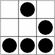
\includegraphics[height=4ex]{logo}}
}
\cfoot{\color{color2}EPS 7008 - Gestão Estratégica da TI}
\rfoot{\color{color2}\thepage}
\renewcommand\headrulewidth{0pt}
\renewcommand\footrulewidth{0pt}

%%% picture on cover page
\usepackage{eso-pic}
\newcommand\BackgroundPic{%
\put(0,0){%
\parbox[b][\paperheight]{\paperwidth}{%
\vfill
\centering

\includegraphics[width=\paperwidth,height=\paperheight,%
keepaspectratio]{cover}%
\vfill
}}}
%%%
% custom titlepage
\makeatletter
\renewcommand{\maketitle}{
\thispagestyle{empty}
\AddToShipoutPicture*{\BackgroundPic}
\ClearShipoutPicture
%
\phantom{a}
\vfill
\phantom{a}\hfill
\begin{tabular}[c]{@{}p{0.7\textwidth}@{}}
      \color{white}\headingfont\LARGE\@title\\[1em]
      \color{white}\headingfont\Large\@author\\[2em]
\end{tabular}
%
\clearpage
}
\makeatother
%%%


%%% fancy boxes
\usepackage{tcolorbox}
\usepackage{wrapfig}
\def\fullboxbegin{
\bigskip
\begin{tcolorbox}[colback=color1,colframe=color1,coltext=white,arc=0mm,boxrule=0pt]
}
\def\fullboxend{\end{tcolorbox}\medskip}
%
\def\leftboxbegin{
\begin{wrapfigure}{l}{0.5\textwidth}
\begin{tcolorbox}[colback=color1,colframe=color1,coltext=white,arc=0mm,boxrule=0pt]
}
\def\leftboxend{
\end{tcolorbox}
\end{wrapfigure}
}
%
\def\rightboxbegin{
\begin{wrapfigure}{r}{0.5\textwidth}
\begin{tcolorbox}[colback=color1,colframe=color1,coltext=white,arc=0mm,boxrule=0pt]
}
\def\rightboxend{
\end{tcolorbox}
\end{wrapfigure}
}
%
\newcounter{frames}
\def\frameboxbegin#1{
\bigskip
\refstepcounter{frames}
\begin{tcolorbox}[colback=white,colframe=color1,arc=0mm,title={\MakeUppercase{\textbf{Frame \arabic{frames}}: #1}}]
}
\def\frameboxend{
\end{tcolorbox}
}
%%%
\ifLuaTeX
  \usepackage{selnolig}  % disable illegal ligatures
\fi

\title{Relatorio da Tarefa 2}
\usepackage{etoolbox}
\makeatletter
\providecommand{\subtitle}[1]{% add subtitle to \maketitle
  \apptocmd{\@title}{\par {\large #1 \par}}{}{}
}
\makeatother
\subtitle{EPS7008 - Gestão Estratégica da TI}
\author{Nome e Sobrenome}
\date{13/06/2022}

\begin{document}
\maketitle

{
\setcounter{tocdepth}{3}
\tableofcontents
}
\hypertarget{instruuxe7uxf5es}{%
\section{Instruções}\label{instruuxe7uxf5es}}

Esta Tarefa 2 servirá para vocês aplicarem os conhecimentos de
visualização de dados e de apresentação das visualizações em formato de
relatório (PDF) e de Dashboard.

Para isto, cada um de vocês deverá escolher um dataset, alguns sites
onde vocês podem localizar potenciais datasets são:
\href{https://www.kaggle.com/datasets}{kaggle},
\href{https://data.fivethirtyeight.com/}{FiveThirtyEight},
\href{https://dados.gov.br/dataset}{Portal Brasileiro de Dados Abertos},
o \href{https://datacatalog.worldbank.org/home}{Open Data do Banco
Mundial} e
\href{https://github.com/rfordatascience/tidytuesday}{tidytuesdday}.
\textbf{Considerando a ampla variedade de dados será portanto,
improvável ter dois datasets identicos.}

Para garantir que não haverão dois datasets iguais, peço-lhes preencher
\href{https://docs.google.com/spreadsheets/d/1nTPGJM0Ulj3v2kfgXYPQsztGDe29fDf4a1FnicAfICY/edit\#gid=0}{esta
planilha} com os dados do dataset escolhido bem como de revisá-la para
verificar os datasets escolhidos pelos colegas e assim evitar
duplicidades.

\textbf{dica}: Podem procurar por assuntos que tenham afinidade ou
curiosidade, quanto mais singular for o dataset, mais divertida e
informativa será a visualização de dados.

A entrega necessariamente exige:

\begin{itemize}
\tightlist
\item
  Apresentação de análises exploratórias, em formato de gráficos
  (principalmente) e tabelas e sua discussão.
\item
  Para as análises exploratórias devem usar-se gráficos diversos
  (revisar material do Datacamp sobre visualização. Podem usar-se vários
  dos tipos de gráficos aprendidos além de outros e também indicadores
  numéricos ou KPIs (p.ex. médias, total de contagens, etc.).
\item
  Construção de dashboard retratando a síntese das informações (gráficas
  e numéricas) mais importantes (usando Flexdashboard e Shiny em R).
\item
  Arquivo \texttt{Rmd} do dashboard
\item
  Relatório em PDF, detalhando todas as ações feitas: limpeza de dados,
  agrupamentos, filtragens etc, bem como as análises e visualização de
  dados.
\end{itemize}

\hypertarget{ruxfabrica}{%
\section{Rúbrica}\label{ruxfabrica}}

A rúbrica a seguir mostra os critérios de avaliação que serão usados no
Moodle.

\begin{longtable}[]{@{}
  >{\raggedright\arraybackslash}p{(\columnwidth - 8\tabcolsep) * \real{0.1757}}
  >{\raggedright\arraybackslash}p{(\columnwidth - 8\tabcolsep) * \real{0.1757}}
  >{\raggedright\arraybackslash}p{(\columnwidth - 8\tabcolsep) * \real{0.1757}}
  >{\raggedright\arraybackslash}p{(\columnwidth - 8\tabcolsep) * \real{0.2838}}
  >{\raggedright\arraybackslash}p{(\columnwidth - 8\tabcolsep) * \real{0.1892}}@{}}
\caption{Criterios da Rúbrica}\tabularnewline
\toprule
\begin{minipage}[b]{\linewidth}\raggedright
Critérios
\end{minipage} & \begin{minipage}[b]{\linewidth}\raggedright
Não concluído
\end{minipage} & \begin{minipage}[b]{\linewidth}\raggedright
Insatisfatório
\end{minipage} & \begin{minipage}[b]{\linewidth}\raggedright
Satisfatório
\end{minipage} & \begin{minipage}[b]{\linewidth}\raggedright
Excelente
\end{minipage} \\
\midrule
\endfirsthead
\toprule
\begin{minipage}[b]{\linewidth}\raggedright
Critérios
\end{minipage} & \begin{minipage}[b]{\linewidth}\raggedright
Não concluído
\end{minipage} & \begin{minipage}[b]{\linewidth}\raggedright
Insatisfatório
\end{minipage} & \begin{minipage}[b]{\linewidth}\raggedright
Satisfatório
\end{minipage} & \begin{minipage}[b]{\linewidth}\raggedright
Excelente
\end{minipage} \\
\midrule
\endhead
\textbf{Uso de gráficos univariados e multivariados} & Não foram
apresentados gráficos (0 pontos) & Os gráficos são pobremente usados ou
não ajudam na interpretação das análises propostas. As explicações não
estão bem fundamentadas nos dados e são incompletas. A análise gráfica e
visual não é exaustiva. Não são gerados insights significativos e nem
informações que ajudem na tomada de decisão. (1 ponto) & Nem todos os
gráficos usados ajudam na interpretação das análises propostas. Ou as
explicações são incompletas ou apenas parcialmente baseadas nos dados. A
análise gráfica e visual é ampla porém não é exaustiva e dá a impressão
que mais poderia ter sido feito. Os insights são tanto quanto óbvios e
não necessariamente ajudam a informar a tomada de decisão. Os recursos
simples do ggplot bem aplicados enquanto os mais complexos não,
apresentando sobreposicões ou legendas mal posicionadas ou não seguindo
outras boas práticas de visualização. (2 pontos) & Os gráficos usados
são adequados para as análises propostas e as explicações são claramente
baseadas nos dados coletados. A análise gráfica e visual é exaustiva -
de qualidade - e ajuda a identificar insights interessantes e
informativos para a tomada de decisão. Há um uso de diversos recursos
simples e complexos do ggplot. E as boas práticas de visualização são
sempre usadas. (3 pontos) \\
\textbf{Uso do dataset fornecido} & O dataset não está limpo, não teve
colunas renomeadas e não reclassifica as colunas de caracteres em outras
mais adequadas. (0 pontos) & O uso do dataset é pobre. Apenas poucas
informações são utilizadas para gerar os gráficos e análises
exploratórias. Quando usados, os dados são usados sem apresentar
sínteses ou agrupamentos que ajudem a lidar com o volume amplo de
informações. Portanto, os gráficos e as análises exploratórias são
pobres pois não ajudam a tirar conclusões relevantes. (1 ponto) & O
dataset é explorado parcialmente. Nem todas as informações nele foram
sintetizadas para serem usadas em sua totalidade ou não se procuraram
formas para agrupar essas informações. Portanto, os gráficos e as
análises exploratórias são parciais porém suficientes como para tirar
conclusões relevantes. Houve uma limpeza adequada dos dados. (2 pontos)
& O dataset é amplamente explorado, de forma que ele é usado por
completo seja para a confecção dos gráficos bem como das análises
exploratórias. Isso inclui um uso exaustivo e de qualidade de todas as
informações (colunas) providas no dataset. Há portanto um cuidado com a
limpeza dos dados, reformatação de colunas e seleção das que de fato
serão usadas. \\
\textbf{Dashboard} & O código fornecido não compila um dashboard. (0
pontos) & O dashboard apresenta sérios problemas de consistência com os
dados (p.ex. Resultados diferentes dos encontrados no relatório). Há
vários problemas estéticos e de funcionamento no dashboard, tais como
controles inoperantes ou produzindo erros e distribuição (layout) mal
planejada e combinação de cores inadequada. (1 ponto) & O dashboard é
relativamente consistente com os dados, mas apresenta alguns problemas
de estética, tais como cores inconsistentes, disposição (layout)
inadequada e elementos (gráficos e números) mal distribuídos ou
pobremente usados. Há controles interativos simples, porém que ajudam
suficientemente o usuário a navegar pelas informações. (2 pontos) & O
dashboard é consistente com os dados analisados, é esteticamente
agradável e segue as boas práticas de construção de dashboards, tais
como paleta de cores previamente definida, disposição (layout) estético
das informações e um mix entre gráficos e números (KPI). Além disso, o
dashboard inclui controles interativos que facilitam a manipulação do
usuário. (3 pontos) \\
\textbf{Qualidade do Relatório} & Não existe relatório, ou o código
fornecido não compila o PDF (0 pontos). & O relatório apresenta vários
problemas de escrita e de formatação no Rmd ou no PDF. Por exemplo,
erros de código que não geram os gráficos no PDF. O relatório não conduz
o leitor ao longo das análises feitas (gráficas e numéricas) e portanto
geram dificuldades para entender como se chegaram às conclusões
apresentadas. (0,33 pontos) & O relatório está bem escrito, porém com
alguns erros de português e/ou formatação no Rmd ou no PDF. O relatório
conduz o leitor ao longo das análises feitas, porém com certas
inconsistências ou falta de clareza, porém sem dificultar demais a
compreensão dos resultados e conclusões apresentadas. (0,66 pontos) &
Relatório bem escrito, sem erros de português e nem de formatação (tanto
no Rmd quanto no PDF) e retratando claramente as análises gráficas e
numéricas. O relatório conduz o leitor ao longo das análises feitas,
ajudando na compreensão dos resultados e conclusões apresentadas. (1
ponto) \\
\bottomrule
\end{longtable}

\end{document}
